\section{object vs artifact}
\label{chapter-scenario-template}

\textbf{Created by:} Perawit Charoenwut \\
\textbf{Modified by:}

\subsection*{Scenario Objective}

An object is constituted of one or more materials. In this scenario, the bfo:Object is related to multiple core:MaterialComponent via the bfo:has continuant part at some. Each core:MaterialComponent is related to a bfo:quality via the bfo:bearerOf.
\subsection*{General Pattern Description}

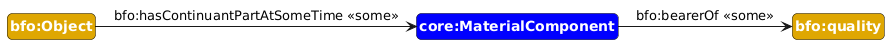
\includegraphics[scale=0.5]{scenarios/object-artifact-material/image/what-is-made-of-schema.png}
A material entity (bfo:MaterialEntity) may be composed of multiple components (iof:Component). The relationships between a material entity and its components are represented using bfo:hasContinuantPartAtSomeTime.

\subsection*{Use Case: Glass Top Steel Table}
A modern table with a tempered glass top and stainless steel frame demonstrates how different materials compose different parts of an object.

\subsubsection*{Use-Case Pattern Description}
The table is a bfo:Object. It has three main material components that are instances of core:MaterialComponent: 
\begin{itemize}
    \item Tempered glass component for the top
    \item Stainless steel rectangle tube component for the frame
    \item Stainless steel round rod component for the legs
    \item Nylon wheels with rubber coating
\end{itemize}

Each component specifies its material type and quality
\subsubsection*{Use-Case Example Data}
\begin{table}[h]
% \caption{}
\label{tab:material-components}
\resizebox{\columnwidth}{!}{%
\begin{tabular}{|l|l|l|l|l|l|l|}
\hline
Component ID & Product ID & Component Type & Material & Quality Type & Quality Value & Unit \\ \hline
TOP001 & TABLE001 & Table Top & Tempered Glass & Thickness & 10 & mm \\
TOP001 & TABLE001 & Table Top & Tempered Glass & Area & 0.8 & m² \\
FRAME001 & TABLE001 & Table Frame & Steel & Length & 100 & cm \\
FRAME002 & TABLE001 & Table Frame & Steel & Length & 80 & cm \\
LEG001 & TABLE001 & Table Leg & Steel & Height & 75 & cm \\
LEG001 & TABLE001 & Table Leg & Steel & diameter & 5 & cm \\
WHEEL001 & TABLE001 & Wheel & Nylon & Diameter & 50 & mm \\ \hline
\end{tabular}%
}
\end{table}

\subsubsection*{Data Mapping}


\subsubsection*{Data Validation}
